\documentclass{beamer}
\usepackage[spanish]{babel}
\usepackage[utf8]{inputenc}
\usepackage{graphicx}
\usepackage{color}
\newtheorem{definicion}{Definición}
\newtheorem{ejemplo}{Ejemplo}

%%%%%%%%%%%%%%%%%%%%%%%%%%%%%%%%%%%%%%%%%%%%%%%%%%%%%%%%%%%%%%%%%%%%%%%%%%%%%%%
\title[Método de Simpson]{\fbox{\fbox{Método de Simpson}}}
\author[Melanie, Nadia, Tania]{Melanie Hernández, Nadia Chinea, Tania Gutiérrez}
\date[17-05-2013]{17 de mayo de 2013}
%%%%%%%%%%%%%%%%%%%%%%%%%%%%%%%%%%%%%%%%%%%%%%%%%%%%%%%%%%%%%%%%%%%%%%%%%%%%%%%

%\usetheme{Madrid}
%\usetheme{Antibes}
%\usetheme{boxes}
%\usetheme{tree}
%\usetheme{classic}
\usetheme{Malmoe}

\usecolortheme{crane}
\useinnertheme{rounded}
\useoutertheme{shadow}
\usefonttheme{serif}

%%%%%%%%%%%%%%%%%%%%%%%%%%%%%%%%%%%%%%%%%%%%%%%%%%%%%%%%%%%%%%%%%%%%%%%%%%%%%%%
\begin{document}
  
%++++++++++++++++++++++++++++++++++++++++++++++++++++++++++++++++++++++++++++++  
\begin{frame}

%\includegraphics[=0.15\textwidth]{fmatesc.eps}
 \hspace*{7.5cm}
 
\includegraphics[width=0.16\textwidth]{logotipo-secundario-ULL.eps}
  \titlepage

  \begin{scriptsize}
    \begin{center}
     Facultad de Matemáticas \\
     Universidad de La Laguna
    \end{center}
  \end{scriptsize}

\end{frame}
%++++++++++++++++++++++++++++++++++++++++++++++++++++++++++++++++++++++++++++++  

%++++++++++++++++++++++++++++++++++++++++++++++++++++++++++++++++++++++++++++++  
\begin{frame}
  \frametitle{Índice}  
  \tableofcontents[pausesections]
\end{frame}
%++++++++++++++++++++++++++++++++++++++++++++++++++++++++++++++++++++++++++++++  




\section{Motivación y Objetivos}


%++++++++++++++++++++++++++++++++++++++++++++++++++++++++++++++++++++++++++++++  
\begin{frame}

\frametitle{Objetivo principal}
 
\begin{block}{}
La intención principal es el planteamiento de un experimento cuyo fin 
es el cálculo del área de una función dada de la forma más precisa posible. 
Interviene un método de integración numérica, por lo tanto conlleva no sólo un aprendizaje en el ámbito informático 
sino que además permite hacer un enfoque matemático 
que obliga a alcanzar una mayor destreza en este campo.

\end{block}
\end{frame}
%++++++++++++++++++++++++++++++++++++++++++++++++++++++++++++++++++++++++++++++  

%++++++++++++++++++++++++++++++++++++++++++++++++++++++++++++++++++++++++++++++  
\begin{frame}

\frametitle{Objetivos}
\begin{block}{}
  \begin{itemize}
  \item Uso del ~\LaTeX y comprensión de todas sus sentencias de una forma ordenada y precisa como se muestra en este informe.
  \item Utilización de un macro de ~\TeX, Beamer, para desarrollar capacidades de relación y exposición de un tema mediante transparencias 
con la intención de transmitir y mostrar de una forma simple lo que hemos aprendido a traducir a ~\LaTeX.
  \item Manejo de Python, lenguaje principal que permitirá la realización del experimento y la obtención de datos.
  \end{itemize}
\end{block}

\end{frame}
%++++++++++++++++++++++++++++++++++++++++++++++++++++++++++++++++++++++++++++++  

\section{Fundamentos Teóricos}


\begin{frame}
\frametitle{Fundamentos Teóricos}
\begin{block}{}
La forma más común a la hora de hallar áreas de funciones es la integral definida.
La integración es un concepto fundamental del cálculo y del análisis matemático. Básicamente, la integral es una generalización 
de la suma de infinitos sumandos,infinitamente pequeños.
\end{block}
\begin{block}{}
 Algunos métodos numéricos son el método de Taylor,Simpson, punto medio, regla del rectángulo,etc. En este caso, utilizaremos el método de Simpson.
\end{block}
\end{frame}

\begin{frame}
\begin{block}{}

\[\int_{-1}^{1} \frac{1}{\sqrt{2\pi}}\text{e}^{\frac{-x^2}{2}} \text{d}x\] 
Para la regla de Simpson existen dos fórmulas cuya elección recae en el tamaño de la acotación, es decir, para un intervalo pequeño, como por ejemplo [-1,1],
se debe utilizar la fórmula simple del método y para una cota superior, como lo es [2,23] es más correcto el uso de la fórmula compuesta de Simpson.
\end{block}

\end{frame}
\begin{frame}
\begin{block}{Fórmulas}
La fórmula simple se define como:
\[\int_{a}^{b} f(x)\text{d}x ~ \frac{b-a}{6}\big[f(a)+4f(m)+f(b)\big]\]\par
 
Por otra parte, la fórmula compuesta aparece como:

\[\int_{a}^{b} f(x)\text{d}x ~ \frac{h}{3}\big[f(x_0)+2\sum_{j=1}{\frac{n}{2-1}} f(x_{2j})+4 \sum_{j=1}{\frac{n}{2}}f(x_{2j-1})+f(x_n)\]

\end{block}

\end{frame}
%++++++++++++++++++++++++++++++++++++++++++++++++++++++++++++++++++++++++++++++  

\section{Procedimiento experimental}

\begin{frame}
\frametitle{Procedimiento experimental}
\begin{block}{}
El experimento se basará en la comparación entre las fórmulas, en el que se realizarán pruebas de tiempo de ejecución de ambas con 
diferentes intervalos,además de distintas reiteraciones en el caso de la compuesta.
Por lo tanto se puede dividir en dos partes.

\end{block}
\end{frame}
%++++++++++++++++++++++++++++++++++++++++++++++++++++++++++++++++++++++++++++++  

\subsection{Descripción de los experimentos}

%++++++++++++++++++++++++++++++++++++++++++++++++++++++++++++++++++++++++++++++  
\begin{frame}
Esta parte del experimento comienza con la creación de un módulo principal que contiene una definición de la función y llamadas al usuario
con la intención de que introduzca los intervalos deseados. Los resultados que se obtienen se guardarán en un fichero que se pedirá también por teclado, 
pudiendo guardar varias ejecuciones en el mismo, es decir, sin que se sobrescriba al usar el mismo nombre.
En un módulo aparte se calculará el tiempo que tarda en ejecutarse cada intervalo y el tiempo que mantiene el cpu.

\begin{ejemplo}
  \begin{itemize}
 \item Con el intervalo [-1,1]
    \item Con el intervalo [-1,4]
    \item Con el intervalo [2,8]
  \end{itemize}
\end{ejemplo}

\end{frame}

\begin{frame}
\begin{block}{}
 En cuanto a la segunda parte, se podría decir que es una ampliación de la primera. Dado que la fórmula compuesta permite realizar el experimento con 
números de reiteraciones diferentes. Se proponen dos programas en los que el número de reiteraciones esté ya asignado, siendo 2 y 4 el número de 
repeticiones que se harán.
Al igual que en la primera parte verán los tiempos trancurridos y los del CPU.
\end{block}
\end{frame}


%++++++++++++++++++++++++++++++++++++++++++++++++++++++++++++++++++++++++++++++  

\subsection{Descripción del material}
%++++++++++++++++++++++++++++++++++++++++++++++++++++++++++++++++++++++++++++++  
\begin{frame}
\frametitle{Hardware y Software}

\begin{ejemplo}
  \begin{enumerate}
\item Tipo de CPU: Pentium(R) Dual-Core  CPU      E5200  @ 2.50GHz 
\pause 
\item cache size: 2048 KB 
\pause
\item CPU speed: 1200.000 Hz 
\pause
\item
vendor ID: GenuineIntel 
\pause
      
  \end{enumerate}
\end{ejemplo}

\end{frame}
%++++++++++++++++++++++++++++++++++++++++++++++++++++++++++++++++++++++++++++++  

\subsection{Resultados obtenidos}
%++++++++++++++++++++++++++++++++++++++++++++++++++++++++++++++++++++++++++++++  
\begin{frame}
\frametitle{Medidas de tiempo y Velocidad}

%------------------------------------------------------------------------------
%--------------------------------------------------------------------------
\begin{table}[!ht]
\begin{center}
\begin{tabular}{|c||c||c|} \hline 
  \textbf{Intervalo} & \textbf{Area}  \\ \hline \hline
[-1,1] &  0693236856881
\\
\hline
[-1,4] & 0.633179114507
\\
\hline

[2,8] & 0.0539969133913
\\
\hline
\hline

\end{tabular}
\end{center}
\caption{Resultados experimentales del calculo del area (formula simple)}
\label{tab:1}
\end{table}


 %--------------------------------------------------------------------------
\begin{table}[!ht]
\begin{center}
\begin{tabular}{|c||c||c|} \hline 
\textbf{Intervalo} & \textbf{Area con iteracion = 4}  \\ \hline \hline
[-1,1] &  0.5813286
\\
\hline
[-1,4] & 0.646540956
\\
\hline

[2,8] & 0.0278711396576
\\
\hline
\hline

\end{tabular}
\end{center}
\caption{Resultados experimentales del calculo del area (formula compuesta)}
\label{tab:2}
\end{table}

%------------------------------------------------------------------------------

\end{frame}
%++++++++++++++++++++++++++++++++++++++++++++++++++++++++++++++++++++++++++++++  
\begin{frame}
 %--------------------------------------------------------------------------
\begin{table}[!ht]
\begin{center}
\begin{tabular}{|c||c||c|} \hline 
\textbf{Intervalo} & \textbf{Tiempo transcurrido}  & \textbf{Tiempo CPU}\\ \hline \hline
[-1,1] &  1.096754 $\text{e}^{-0.5}$& 0.0
\\
\hline
[-1,4] & 1.2159347$\text{e}^{-0.5}$ & 0.0
\\
\hline

[2,8] & 1.096725 $\text{e}^{-0.5}$& 0.0
\\
\hline
\hline

\end{tabular}
\end{center}
\caption{Resultados experimentales de tiempo(formula simple)}
\label{tab:3}
\end{table}

 %--------------------------------------------------------------------------
\begin{table}[!ht]
\begin{center}
\begin{tabular}{|c||c||c|} \hline 
\textbf{Intervalo} & \textbf{Tiempo transcurrido}  & \textbf{Tiempo CPU}\\ \hline \hline
[-1,1] &  9.059906$\text{e}^{-0.5}$ & 0.0
\\
\hline
[-1,4] & 1.001358 $\text{e}^{-0.5}$& 0.0
\\
\hline

[2,8] & 7.867813 $\text{e}^{-0.6}$& 0.0
\\
\hline
\hline

\end{tabular}
\end{center}
\caption{Resultados experimentales de tiempo (formula compuesta)}
\label{tab:2}
\end{table}
\end{frame}

%++++++++++++++++++++++++++++++++++++++++++++++++++++++++++++++++++++++++++++++  
\begin{frame}
\frametitle{Representaciones de las funciones}

%------------------------------------------------------------------------------

\begin{figure}[!th]
\begin{center}
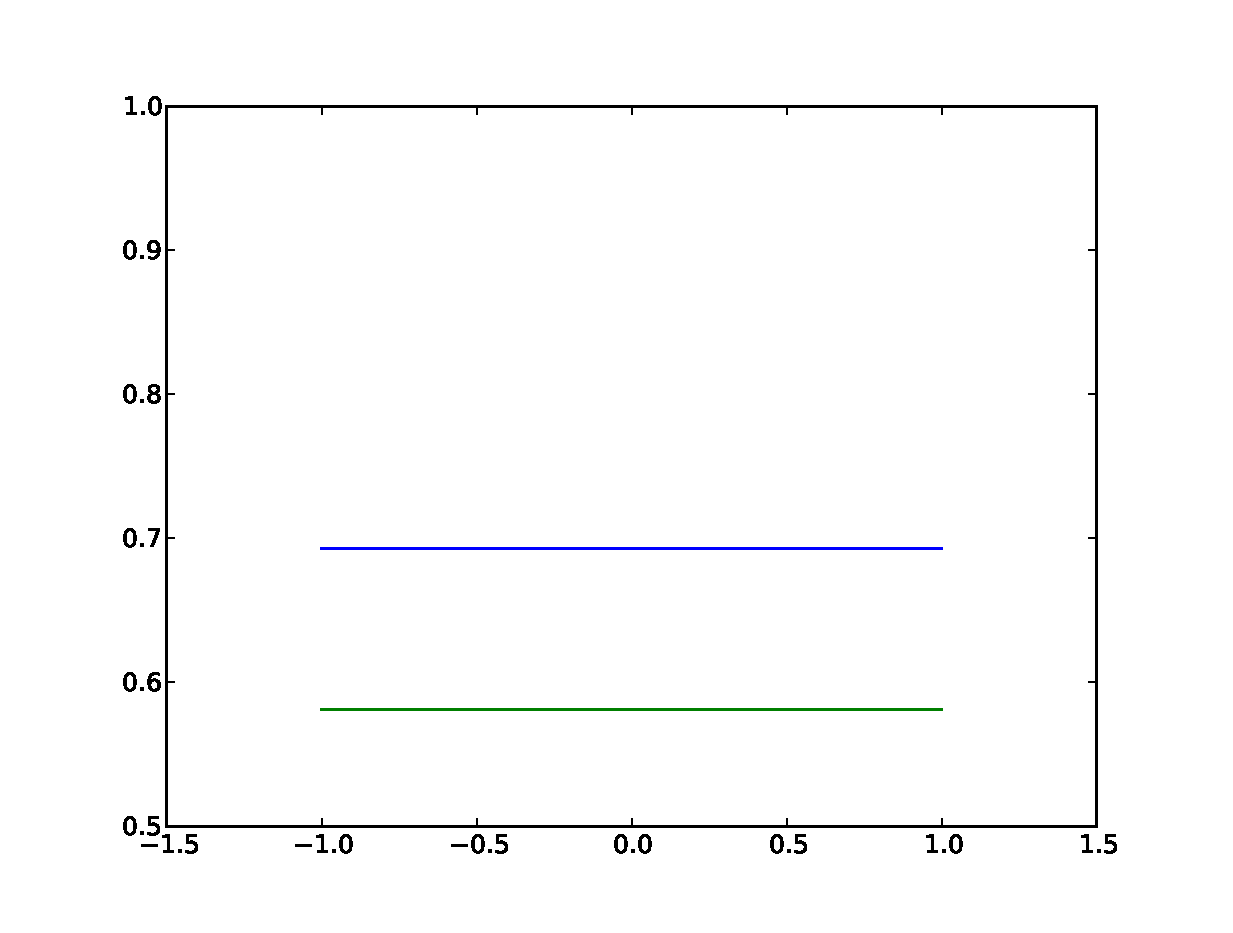
\includegraphics[width=0.75\textwidth]{1intervalo.eps}
\caption{Intervalo [-1,1]}
\label{fig:1}
\end{center}
\end{figure}
\end{frame}

\begin{frame}
 \begin{figure}[!th]
\begin{center}
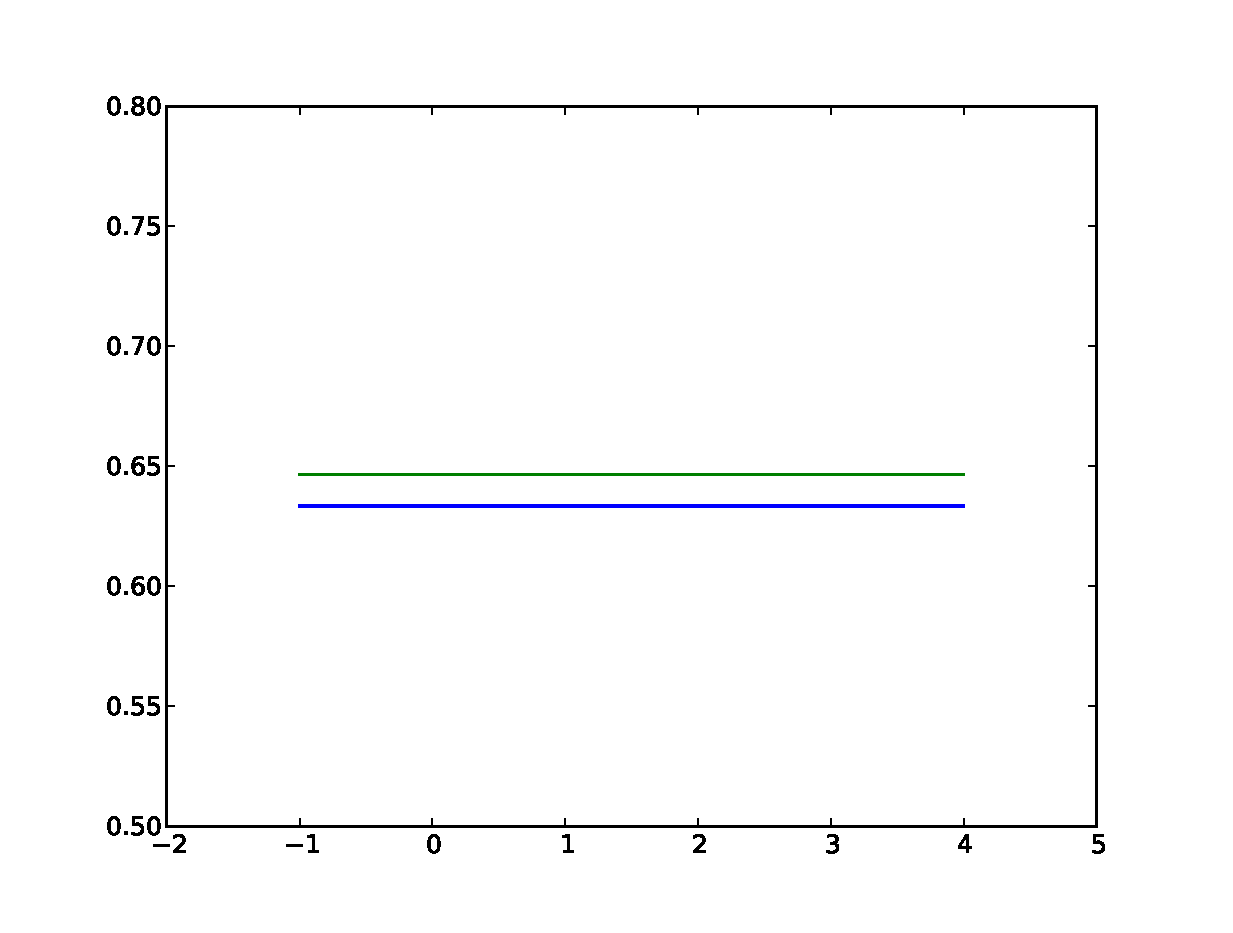
\includegraphics[width=0.75\textwidth]{2intervalo.eps}
\caption{Intervalo [-1,4]}
\label{fig:2}
\end{center}
\end{figure}
\end{frame}
\begin{frame}
 \begin{figure}[!th]
\begin{center}
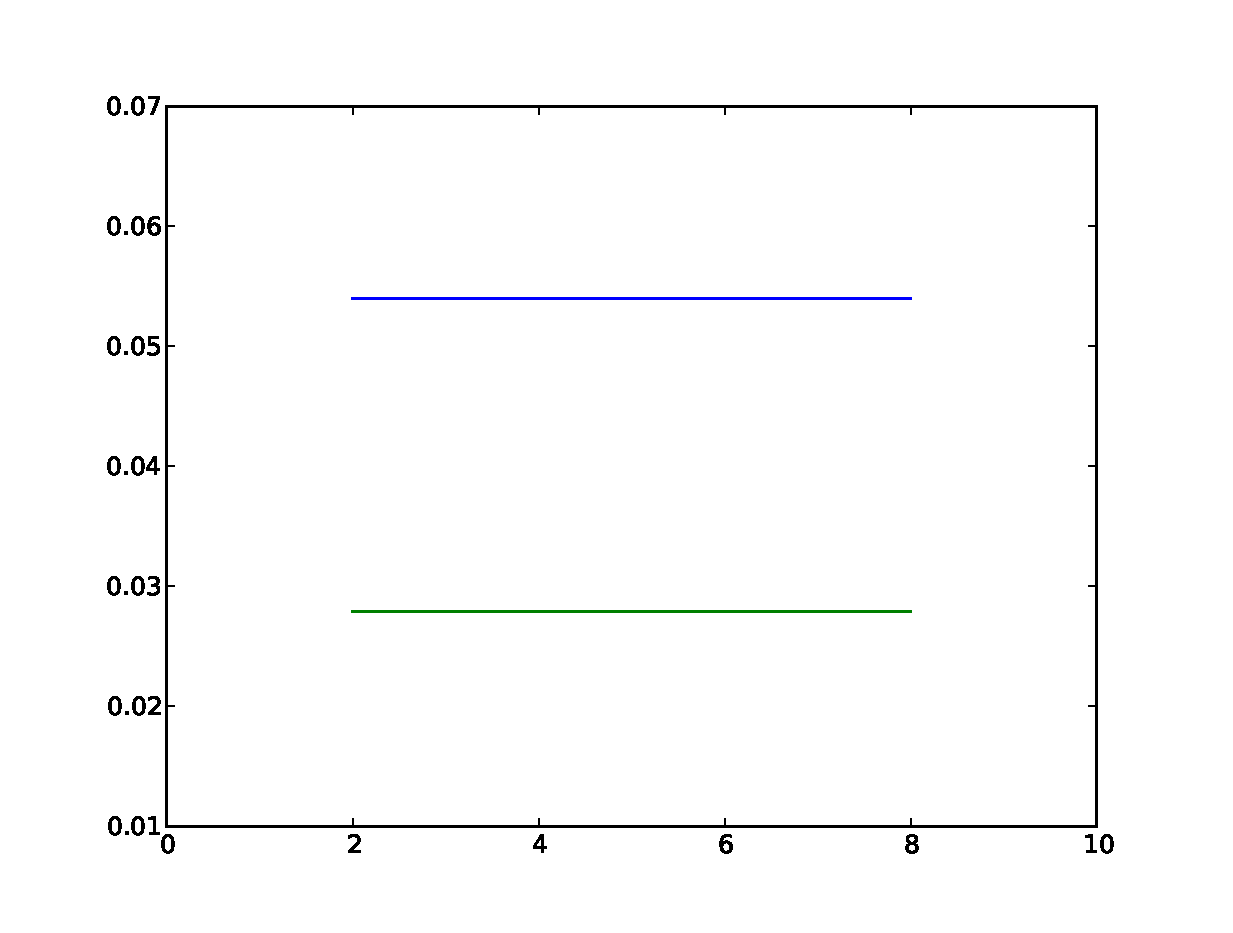
\includegraphics[width=0.75\textwidth]{3intervalo.eps}
\caption{Intervalo [2,8]}
\label{fig:3}
\end{center}
\end{figure}
\end{frame}


%------------------------------------------------------------------------------


%++++++++++++++++++++++++++++++++++++++++++++++++++++++++++++++++++++++++++++++  

\subsection{Análisis de los resultados}
\begin{frame}
\begin{block}{}
De las gráficas podemos decir que con los intervalos [-1,1] y [2,8], las rectas que 
se forman están más alejadas entre sí que en el intervalo que podríamos considerar ni grande ni pequeño. 
Se ha experimentado con el tiempo transcurrido para el tratamiento del método y con el de ejecución de la CPU. Como sabemos, el tiempo 
transcurrido durante la ejecución del programa varía dependiendo de la computadora que se use, aún así podemos apreciar que es mayor al realizar la fórmula 
compuesta debido a que las reiteraciones hacen que el programa se retase.
En cuanto al tiempo de la CPU, no varía en absoluto en ninguno de los intervalos porque la respuesta de la CPU es inmediata.
\end{block}


\end{frame}
\section{Conclusiones}

%++++++++++++++++++++++++++++++++++++++++++++++++++++++++++++++++++++++++++++++  
\begin{frame}
\frametitle{Conclusiones}

El objetivo de este trabajo ha sido la confección de un informe redactado en código ~\LaTeX, y unas transparencias en Beamer con este mismo lenguaje. 
Cabe decir, que el lenguaje de programación con el que se ha confeccionado el experimento ha sido el python.
Hemos obtenido la verificación de que los intervalos menores se usan para la fórmula simple y 
que los mayores para la fórmula compuesta.
También hemos visto que en los programas en los que intervienen definiciones de funciones no muy complejas el tiempo de la CPU es mínimo.
Se puede concluir diciendo que hemos obtenido facilidades a la hora de creación de códigos para resolución de problemas, ademas de haber 
logrado aumentar las capacidades que ya se tenían con ~\LaTeX
\end{frame}
%++++++++++++++++++++++++++++++++++++++++++++++++++++++++++++++++++++++++++++++  
%+++++++++++++++++++++++++++++++++++++++++++++++++++++++++++++++++++++++++++  

\end{document}